\documentclass{beamer}
\usepackage[utf8]{inputenc}

\usetheme{Madrid}
\usecolortheme{default}
\usepackage{amsmath,amssymb,amsfonts,amsthm}
\usepackage{txfonts}
\usepackage{tkz-euclide}
\usepackage{listings}
\usepackage{adjustbox}
\usepackage{array}
\usepackage{tabularx}
\usepackage{gvv}
\usepackage{lmodern}
\usepackage{circuitikz}
\usepackage{tikz}
\usepackage{graphicx}
\usepackage{mathtools}
\setbeamertemplate{page number in head/foot}[totalframenumber]

\usepackage{tcolorbox}
\tcbuselibrary{minted,breakable,xparse,skins}



\definecolor{bg}{gray}{0.95}
\DeclareTCBListing{mintedbox}{O{}m!O{}}{%
  breakable=true,
  listing engine=minted,
  listing only,
  minted language=#2,
  minted style=default,
  minted options={%
    linenos,
    gobble=0,
    breaklines=true,
    breakafter=,,
    fontsize=\small,
    numbersep=8pt,
    #1},
  boxsep=0pt,
  left skip=0pt,
  right skip=0pt,
  left=25pt,
  right=0pt,
  top=3pt,
  bottom=3pt,
  arc=5pt,
  leftrule=0pt,
  rightrule=0pt,
  bottomrule=2pt,
  toprule=2pt,
  colback=bg,
  colframe=orange!70,
  enhanced,
  overlay={%
    \begin{tcbclipinterior}
    \fill[orange!20!white] (frame.south west) rectangle ([xshift=20pt]frame.north west);
    \end{tcbclipinterior}},
  #3,
}
\lstset{
    language=C,
    basicstyle=\ttfamily\small,
    keywordstyle=\color{blue},
    stringstyle=\color{orange},
    commentstyle=\color{green!60!black},
    numbers=left,
    numberstyle=\tiny\color{gray},
    breaklines=true,
    showstringspaces=false,
}

\title 
{4.13.66}
\date{October 10, 2025}


\author 
{Vivek K Kumar - EE25BTECH11062}



\begin{document}


\frame{\titlepage}
\begin{frame}{Question}
A straight line $L$ with negative slope passes through the point $\brak{8, 2}$ and cuts the
positive coordinate axes at points $P$ and $Q$. Find the absolute minimum value of
$OP + OQ$, as $L$ varies, where $O$ is the origin.
\end{frame}

\begin{frame}{Variables used}
\begin{align}
\end{align}
\begin{table}[H]    
  \centering
  \begin{tabular}{|c|c|}
\hline
\textbf{Name} & \textbf{Value} \\ \hline
$\vec{A}$ & $\myvec{2 & 1 \\0 & 3}$ \\ \hline
\end{tabular}

  \caption{Variables used}
  \label{tab:4.13.66}
\end{table}

\end{frame}

\begin{frame}{Solution}
It is known that 
\begin{align}
    \vec{e_1}^\top\vec{P} = 0 \\
    \vec{e_2}^\top\vec{Q} = 0
\end{align}

Given line $L$ can be represented as 
\begin{align}
    \vec{x} = \vec{h} + k\vec{m} \\
    \vec{e_1}^\top\vec{P} = \vec{e_1}^\top\vec{h} + k_1\vec{e_1}^\top\vec{m} \\
    k_1 = -\frac{\vec{e_1}^\top\vec{h}}{\vec{e_1}^\top\vec{m}} \\
    \vec{P} = \vec{h} - \frac{\vec{e_1}^\top\vec{h}}{\vec{e_1}^\top\vec{m}}\vec{m}
\end{align}
\end{frame}
\begin{frame}{Solution}
\begin{align}
\vec{e_2}^\top\vec{Q} = \vec{e_2}^\top\vec{h} + k_2\vec{e_2}^\top\vec{m} \\
k_2 = -\frac{\vec{e_2}^\top\vec{h}}{\vec{e_2}^\top\vec{m}} \\
\vec{Q} = \vec{h} - \frac{\vec{e_2}^\top\vec{h}}{\vec{e_2}^\top\vec{m}}\vec{m} \\
\end{align}
\end{frame}

\begin{frame}{Solution}
Substituting values
\begin{align}
    \vec{P} &= \myvec{8 \\ 2} - 8\myvec{1 \\ -m} \\
            &= \myvec{0 \\ 2+8m} \\
    \vec{Q} &= \myvec{8 \\ 2} - \frac{2}{m}\myvec{1 \\ -m} \\
            &= \myvec{8 + \frac{2}{m} \\ 0}
\end{align}
\end{frame}

\begin{frame}{Solution}
We have to find the minimum of $\norm{\vec{P}} + \norm{\vec{Q}}$
\begin{align}
    \norm{\vec{P}} + \norm{\vec{Q}} &= 2 + 8m + 8 + \frac{2}{m} \\
    &= 10 + 8m + \frac{2}{m}
\end{align}
Applying AM-GM inequality
\begin{align}
    \frac{8m + \frac{2}{m}}{2} &\geq \sqrt{8m .\frac{2}{m}} \\
    &\geq 4\\
    \implies 10 + 8m + \frac{2}{m} &\geq 18
\end{align}
Hence we can write
\begin{align}
    \norm{\vec{P}} + \norm{\vec{Q}} \geq 18
\end{align}
Hence, $min\brak{\norm{\vec{P}} + \norm{\vec{Q}}} = 18$
\end{frame}

\begin{frame}[fragile]
    \frametitle{Python - Importing libraries and checking system}
    \begin{lstlisting}
import sys
import numpy as np
import numpy.linalg as LA
import matplotlib.pyplot as plt
import matplotlib.image as mpimg
import math

from libs.line.funcs import *
from libs.triangle.funcs import *
from libs.conics.funcs import circ_gen

import subprocess
import shlex

print('Using termux?(y/n)')
y = input()
\end{lstlisting}
\end{frame}

\begin{frame}[fragile]
    \frametitle{Python - Setting up Variables and plotting the line equation}
    \begin{lstlisting}
A = np.array([8, 2]).reshape(-1,1)
m = np.array([1, -1/2]).reshape(-1,1)

p_l1 = line_gen(A-8*m, A+4*m)

plt.plot(p_l1[0, :], p_l1[1, :], label = 'Line with min OP+OQ')

pts = np.block([A-8*m, A+4*m, A])
labels = ['P(0,6)', 'Q(12,0)', 'A(8,2)']
plt.scatter(pts[0, :], pts[1, :])
for i, txt in enumerate(labels):
        plt.annotate(txt, (pts[0, i], pts[1, i]), textcoords="offset points", xytext=(20,5), ha='center')
\end{lstlisting}
\end{frame}

\begin{frame}[fragile]
    \frametitle{Python - Setting up plot and labeling axes}
    \begin{lstlisting}
ax = plt.gca()
ax.spines['top'].set_color('none')
ax.spines['bottom'].set_position('zero')
ax.spines['right'].set_color('none')
ax.spines['left'].set_position('zero')
plt.xlabel('x')
plt.ylabel('y')
plt.legend(loc='best')
plt.grid()
plt.axis('equal')
\end{lstlisting}
\end{frame}

\begin{frame}[fragile]
    \frametitle{Python - Saving figure and opening it}
    \begin{lstlisting}
fig.savefig('../figs/fig.png')
print('Saved figure to ../figs/fig.png')

if(y == 'y'):
    subprocess.run(shlex.split('termux-open ../figs/fig.png'))
else:
    subprocess.run(["open",  "../figs/fig.png"])
    \end{lstlisting}
\end{frame}


\begin{frame}{Plot-Using only Python}
    \centering
    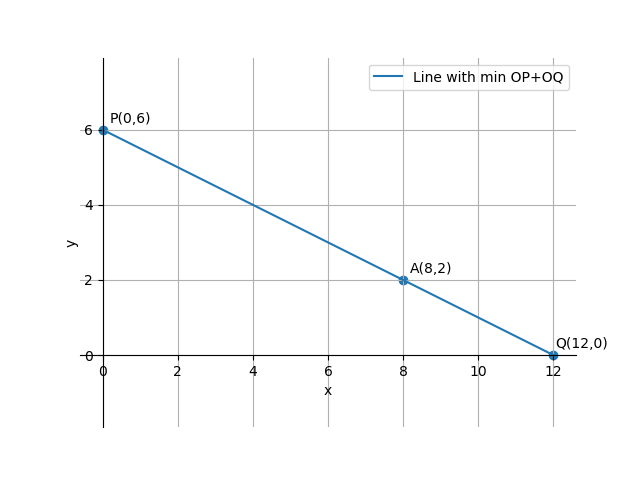
\includegraphics[width=\columnwidth, height=0.8\textheight, keepaspectratio]{../figs/fig.png}     
\end{frame}

\begin{frame}[fragile]
    \frametitle{C Code (0) - Importing libraries}

    \begin{lstlisting}
#include <stdio.h>
#include <stdlib.h>
#include <string.h>
#include <math.h>
#include <sys/socket.h>
#include <netinet/in.h>
#include <unistd.h>
#include "libs/matfun.h"
#include "libs/geofun.h"
    \end{lstlisting}
\end{frame}
\begin{frame}[fragile]
    \frametitle{C Code (1) - Function to Generate Points on a Line}

    \begin{lstlisting}

void point_gen(FILE *p_file, double **A, double **B, int rows, int cols, int npts){
    for(int i = 0; i <= npts; i++){
     double **output = Matadd(A, Matscale(Matsub(B, A, rows, cols), rows, cols, (double)i/npts), rows, cols);
     fprintf(p_file, "%lf, %lf\n", output[0][0], output[1][0]);
     freeMat(output, rows);
    }
}

    \end{lstlisting}
\end{frame}


\begin{frame}[fragile]
    \frametitle{C Code (2) - Function to write points b/w given points to a file}

    \begin{lstlisting}
void write_points(double x1, double y1, double x2, double y2, int npts){
    int m = 2;
    int n = 1;

    double **A = createMat(m, n);
    double **B = createMat(m, n);
    double **C = createMat(m, n);

    A[0][0] = x1-8*x2;
    A[1][0] = y1-8*y2;
    \end{lstlisting}
\end{frame}
\begin{frame}[fragile]
    \frametitle{C Code (2) - Function to write points b/w given 2 points to a file}

    \begin{lstlisting}
    B[0][0] = x1+4*x2;
    B[1][0] = y1+4*y2;

    FILE *p_file;
    p_file = fopen("plot.dat", "w");
    if(p_file == NULL)
        printf("Error opening one of the data files\n");

    point_gen(p_file, A, B, m, n, npts);

    freeMat(A, m);
    freeMat(B, m);

    fclose(p_file);
}
    \end{lstlisting}
\end{frame}

\begin{frame}[fragile]
    \frametitle{Python Code (0) - Importing libraries and checking system}
    \begin{lstlisting}
import numpy as np
import matplotlib.pyplot as plt
import ctypes
import os
import sys
import subprocess
import math

print('Using termux? (y/n)')
termux = input()
\end{lstlisting}
\end{frame}

\begin{frame}[fragile]
    \frametitle{Python Code (1) - Using Shared Object}
    \begin{lstlisting}
lib_path = os.path.join(os.path.dirname(__file__), 'plot.so')
my_lib = ctypes.CDLL(lib_path)

my_lib.write_points.argtypes = [ctypes.c_double, ctypes.c_double, ctypes.c_double, ctypes.c_double, ctypes.c_int]
my_lib.write_points.restype = None
A = np.array([8, 2]).reshape(-1, 1)
m = np.array([1, -1/2]).reshape(-1, 1)
npts = 20000
\end{lstlisting}
\end{frame}

\begin{frame}[fragile]
    \frametitle{Python Code (2) - Loading points and plotting them}
    \begin{lstlisting}
my_lib.write_points(A[0][0], A[1][0], m[0][0], m[1][0], npts)

labels = ['Line with min OP+OQ']
point_labels = ['P(0, 6)', 'Q(12, 0)', 'A(8,2)']
pts = np.block([A-8*m, A+4*m, A])

for i,label in enumerate(labels):
    points = np.loadtxt('plot.dat', delimiter = ',', usecols=(0,1))[i*(npts+1):(i+1)*(npts+1)]
    plt.plot(points[:, 0], points[:, 1], label = label)

for i,label in enumerate(point_labels):
    plt.annotate(label, (pts[0,i],pts[1,i]), textcoords="offset points", xytext=(20,5),ha='center')
\end{lstlisting}
\end{frame}

\begin{frame}[fragile]
    \frametitle{Python Code (3) - Setting up plot and labeling axes}
    \begin{lstlisting}
ax = plt.gca()
ax.spines['top'].set_color('none')
ax.spines['bottom'].set_position('zero')
ax.spines['right'].set_color('none')
ax.spines['left'].set_position('zero')
plt.xlabel('x')
plt.ylabel('y')
plt.legend(loc='best')
plt.grid()
plt.axis('equal')
    \end{lstlisting}
\end{frame}

\begin{frame}[fragile]
    \frametitle{Python Code (4) - Saving and displaying plot}
    \begin{lstlisting}
fig.savefig('../figs/fig2.png')
print('Saved figure to ../figs/fig2.png')

if(termux == 'y'):
    subprocess.run(shlex.split('termux-open ../figs/fig2.png'))
else:
    subprocess.run(["open",  "../figs/fig2.png"])
\end{lstlisting}
\end{frame}

\begin{frame}{Plot-Using Both C and Python}
    \centering
    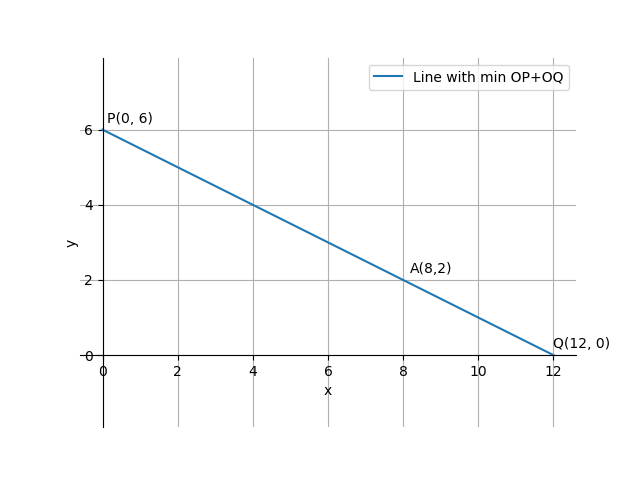
\includegraphics[width=\columnwidth, height=0.8\textheight, keepaspectratio]{../figs/fig2.png}     
\end{frame}

\end{document}